\subsection{Clustering using \acs*{optics}}\label{subsec:impl-optics}

\begin{figure}[htp] % htp = hier (h), top (t), oder auf einer eigenen Seite (p).
    \centering
    \includesvg[width=0.5\textwidth]{images/OPTICS/OPTICS_procedure.svg}
    \caption[\ac{optics} procedure]{The first page of each document is converted to an image.
    The image is preprocessed, i.e. conversion to greyscale and resizing.
    }
    \label{fig:OPTICS_procedure}
\end{figure}

Similar to the approach from \citeauthor{OPTICS1999}, \ac{optics} is used to cluster the images of the first page of documents in this work.
The procedure is displayed in \autoref{fig:OPTICS_procedure}.
There were two different preprocessing approaches:
\begin{enumerate}
    \item \label{pt:32}The images were first preprocessed to 32x32 normalized greyscale pixels (cf. \cite{OPTICS1999}) as visualized in \autoref{fig:preprocessed_docs_32x32}
    and afterwards compressed to 13-dimensional vectors using \ac{pca}.
    \item \label{pt:eigendocs}The technique \eigendocs{} from \autoref{subsec:eigenface} 
    was used to compress the images to 13-dimensional normalized greyscale images as displayed in \autoref{fig:preprocessed_docs_eigendocs}.
\end{enumerate}


% preprocessed images
\begin{figure}[htp] % htp = hier (h), top (t), oder auf einer eigenen Seite (p).
    \centering
    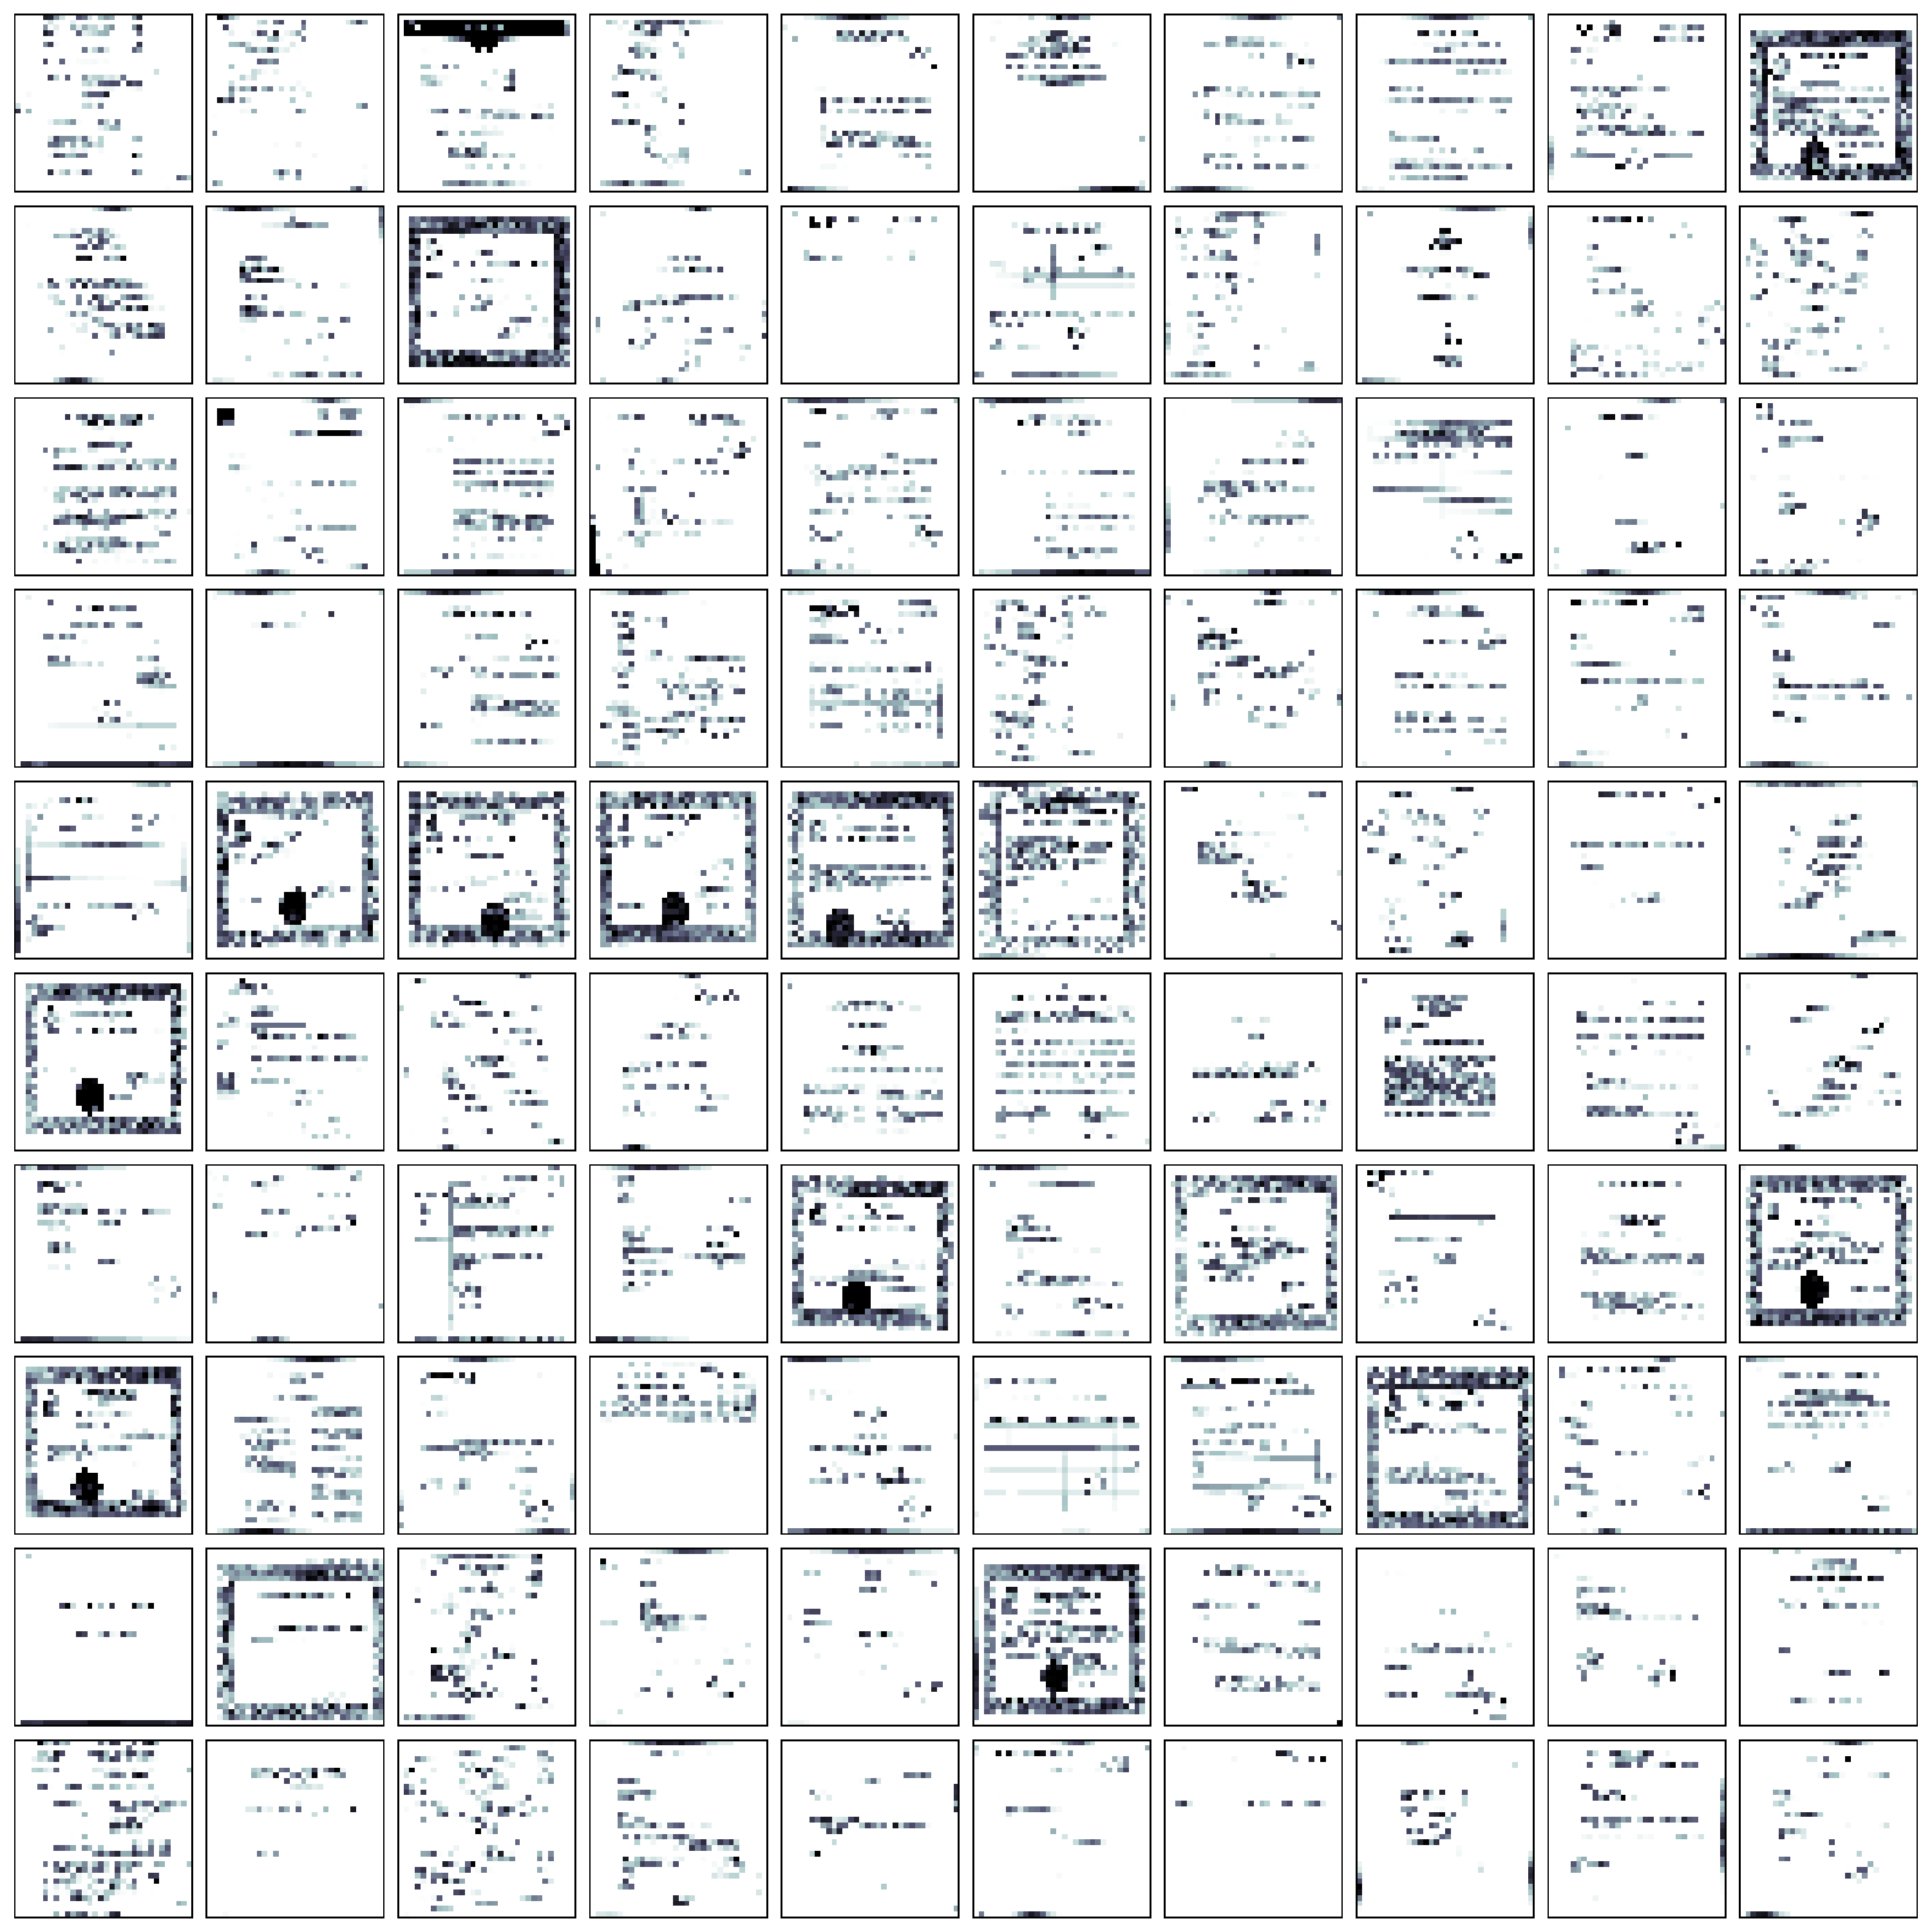
\includegraphics[width=0.4\textwidth]{images/OPTICS/32x32/preprocessed_docs.pdf}
    \caption[Preprocessing to 32x32 normalized greyscale pixels]{Preprocessing of 100 documents to 32x32 normalized greyscale pixels.
    }
    \label{fig:preprocessed_docs_32x32}
\end{figure}


\begin{figure}[htp] % htp = hier (h), top (t), oder auf einer eigenen Seite (p).
    \centering
    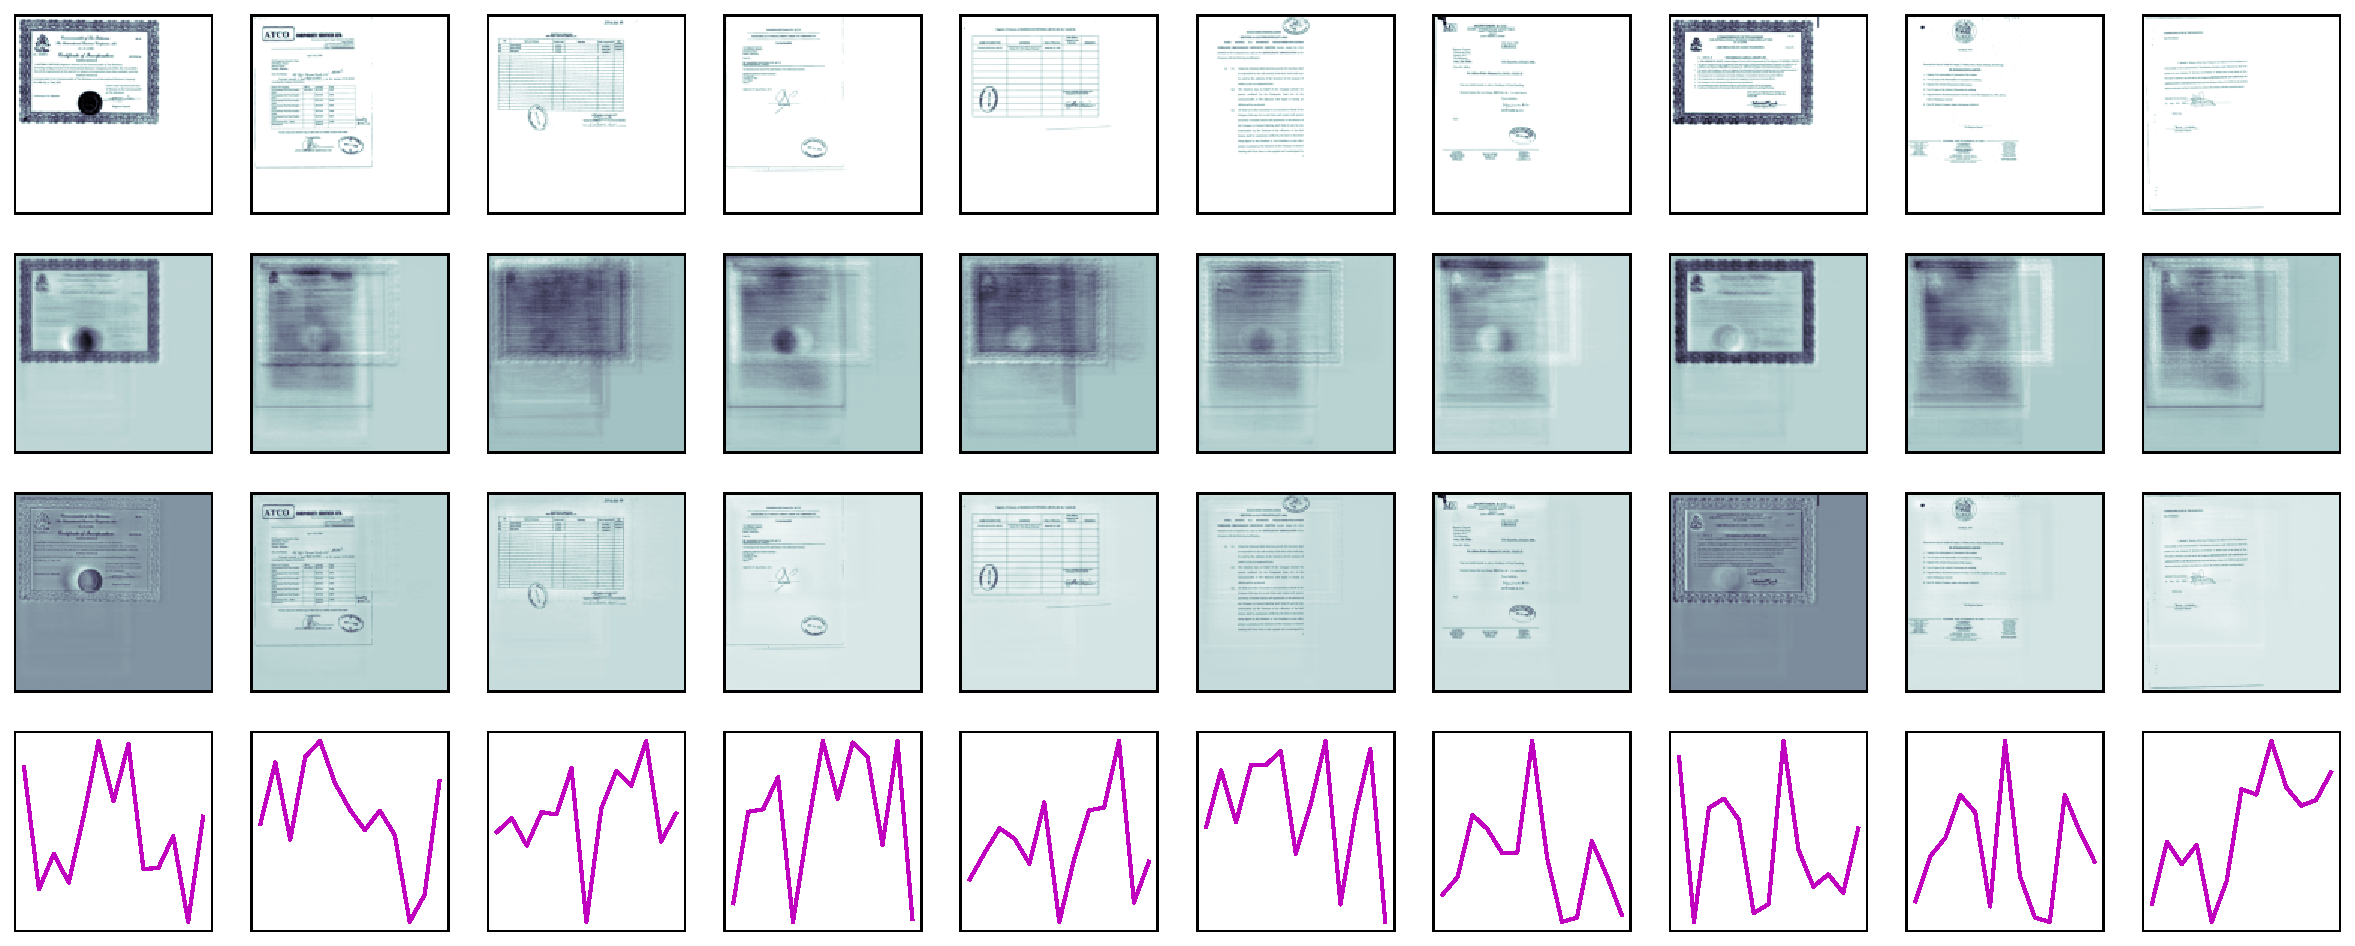
\includegraphics[width=0.7\textwidth]{images/Eigendocs/transformation/eigendocs.pdf}
    \caption[Preprocessing 10 randomly selected documents from the test set]{10 randomly selected documents from the test set.
    The number of images in the test set is 561, while the \ac{pca} model was fit to 1680 training images.
    The original images are displayed in the first row.
    The second row shows the reconstruction from their compressed version in the fourth row.
    The third row shows the reconstruction error, i.e. the difference between the reconstructed and the original image.
    The last row presents the greyscale values of the compressed 13-dimensional image as a line.
    }
    \label{fig:preprocessed_docs_eigendocs}
\end{figure}

The reachability distance ordered by \ac{optics} is displayed in \autoref{fig:reachability_plots}.
%The resulting clusters are displayed in \autoref{fig:optics_cluster}.

% reachability plot
\begin{figure}%
    \centering
    \subfloat[\centering The reachability plot of the documents preprocessed according to \autoref{pt:32} (cf. \cite{OPTICS1999}).]{{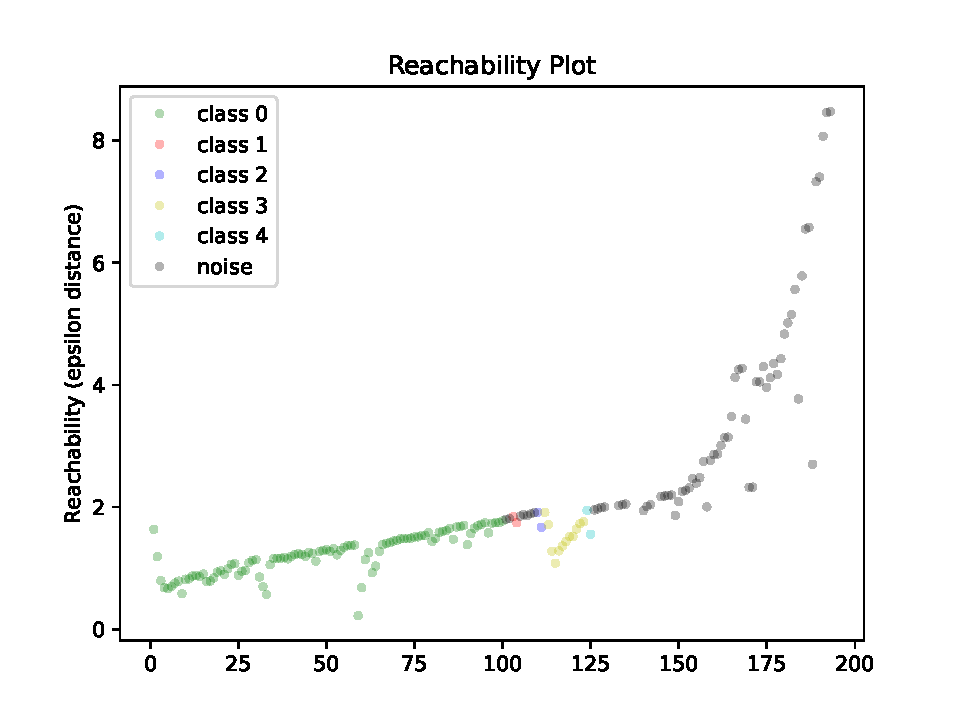
\includegraphics[width=5cm]{images/OPTICS/32x32/reachability_plot_32x32_pca_13dim.pdf} }}%
    \qquad
    \subfloat[\centering The reachability plot of the documents preprocessed according to \autoref{pt:eigendocs} (i.e. \eigendocs{}).]{{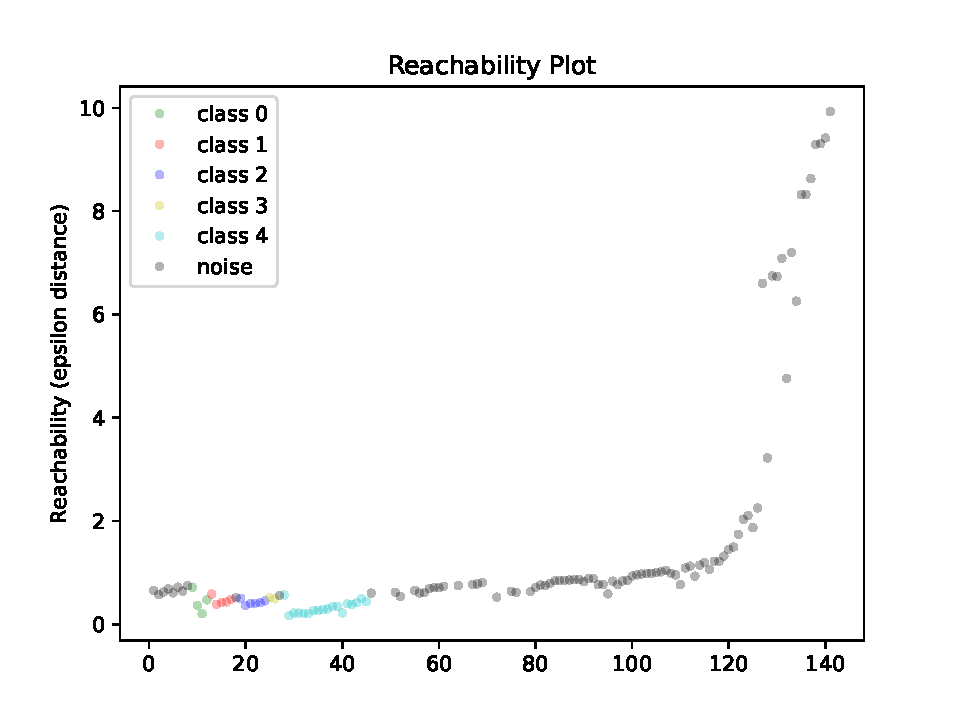
\includegraphics[width=5cm]{images/OPTICS/eigendocs/reachability_plot_13dim_eigendocs.pdf} }}%
    \caption[Reachability distances]{The plot was created using the \ac{optics} algorithm from the Python library scikit-learn.
    It shows the reachability distance of each document to its predecessor in the order list.}%
    \label{fig:reachability_plots}%
\end{figure}

% code
The configurations used when initializing an \ac{optics} model greatly influence the clusters returned.
The parameter \texttt{max\_eps} is infinity by default but can be specified by the user to reduce complexity and runtime.
According to literature, \texttt{max\_eps} should be big enough to include almost all points in a cluster.
The way the reachability plot is used to extract clusters is dependent on the \texttt{cluster\_method}. 
One can choose either \texttt{dbscan} or \texttt{xi} as a clustering method.
The parameters \texttt{min\_samples} and \texttt{eps} influence the cluster sizes and number of clusters found for a given clustering approach.
The value of \texttt{eps} defines the distance between two points to still be considered neighbours 
and can be chosen by consulting the reachability plot.
The code to initialize an exemplary \ac{optics} model is displayed in \lst{lst:optics_model}.

\begin{listing}[htp]
    \begin{minted}{python3}
        optics_model = OPTICS(cluster_method='dbscan', min_samples=2, max_eps=10, 
            eps=0.5)
    \end{minted}
    \caption[Initialization of the \ac{optics} model]{Initialization of the \ac{optics} model.
    The minimum number of samples \texttt{min\_samples} in a cluster corresponds to \textit{minPts}.
    }
    \label{lst:optics_model}
\end{listing}
